\chapter{Vorstudie}\label{Vorstudie}
%%%%%%%%%%%%%%%%%%%%%%%%%%%%%%%%%%%%%%%%%%%%%%%%%%%%%%%%%%%%%%%%%%%%%%%%%%%%%%%%
%Florian-Note:
%Hier würde ich dann als Überleitung erst mal drauf eingehen, wie die existierenden Arbeiten das Design der Vorstudie beeinflusst haben, also z.T. das, was Du jetzt grade in Kapitel 4 schreibst..
%%%%%%%%%%%%%%%%%%%%%%%%%%%%%%%%%%%%%%%%%%%%%%%%%%%%%%%%%%%%%%%%%%%%%%%%%%%%%%%%
%vorüberlegung mit - altes projekt aufsetzen, neues projekt machen?
%\todotext{Übergang - wie haben die Arbeiten das Design der Vorstudie beeinflusst?}\\
%\todotext{ist teilweise schon im kap.4}\\
%Anforderungsanalyse
Zu Beginn war es wichtig eine Anforderungsanalyse durchzuführen. Deshalb musste analysiert werden, in welchem Rahmen sich meine Arbeit bewegen sollte. Es bestanden die Optionen, ein fertiggestelltes Projekt anzupassen und zu verbessern oder ein vollkommen eigenes System zu entwickeln.
\\
Um zu erproben, wie ein bereits fertiges System funktioniert und wie es von Studenten und Mitarbeitern der Medienfakultät der BUW aufgenommen werden würde, habe ich ein bereits vorhandenes Projekt verwendet und in der Praxis getestet.
Da das Hermes System schon relativ alt war und hauptsächlich für PDA's entworfen wurde, kam es für diesen Test nicht in Frage.
Die Entscheidung fiel auf die zweite Version des NetBoards Projekts\cite{netboards:website}, da dieses Projekt das aktuellste war.
\section{NetBoards Experiment}\label{NetBoards Experiment}
%\cite{apache:website}
Als Grundlage für mein Experiment diente ein virtueller Debian-Linux Server mit 1,5GHz AMD CPU und 2GB RAM auf dem Apache2 als Webserver und Python2 für serverseitige Scripts liefen. Das öffentlich zugängliche NetBoards2 Projekt wurde installiert und konfiguriert.
\\
Nachdem der Server eingerichtet war, stellte sich die Frage, was als Anzeigegerät dienen sollte. Das originale Projekt von E. Wood wurde für 22 Zoll Monitore mit Touch-Oberfläche entworfen. Diese wurden vertikal neben die Büroeingänge gehängt.
\\
Da für mein Experiment nicht die notwendigen Ressourcen vorhanden waren, um den genauen Versuchsaufbau nachzuempfinden, fiel die Wahl des Anzeigegerätes auf einen kostengünstigen Tablet-PC.
\\
%\todotext{was war das nochmal für ein tablet? 10Zoll? Spezifikationen angeben}
Dies war ein 10 Zoll Tablet mit 1GHz Cortex A8 Dual Core CPU, 1GB RAM und Android Version 4.4.
\\
Damit die Benutzer nicht mit den auf dem Gerät installierten Applikationen interagieren konnten, wurde eine Kiosk-Applikation\footurl{http://www.android-kiosk.com}{10.12.2015} installiert.
Diese App schränkt die Interaktionsmöglichkeiten der Nutzer nur auf eine ausgewählte Webseite ein. Nur der Administrator des Gerätes hatte die Möglichkeit, diese zu ändern oder die Applikation ganz zu beenden.
\\
Ein weiteres Problem war die Befestigung des Displays.
Ich entschied mich dafür, das Tablet an den bereits vorhanden Türschildern anzubringen \abb{img:Versuchsaufbau}.
\begin{figure}[h!]
  \centering
    \subfigure[Ein typisches Türschild]{
      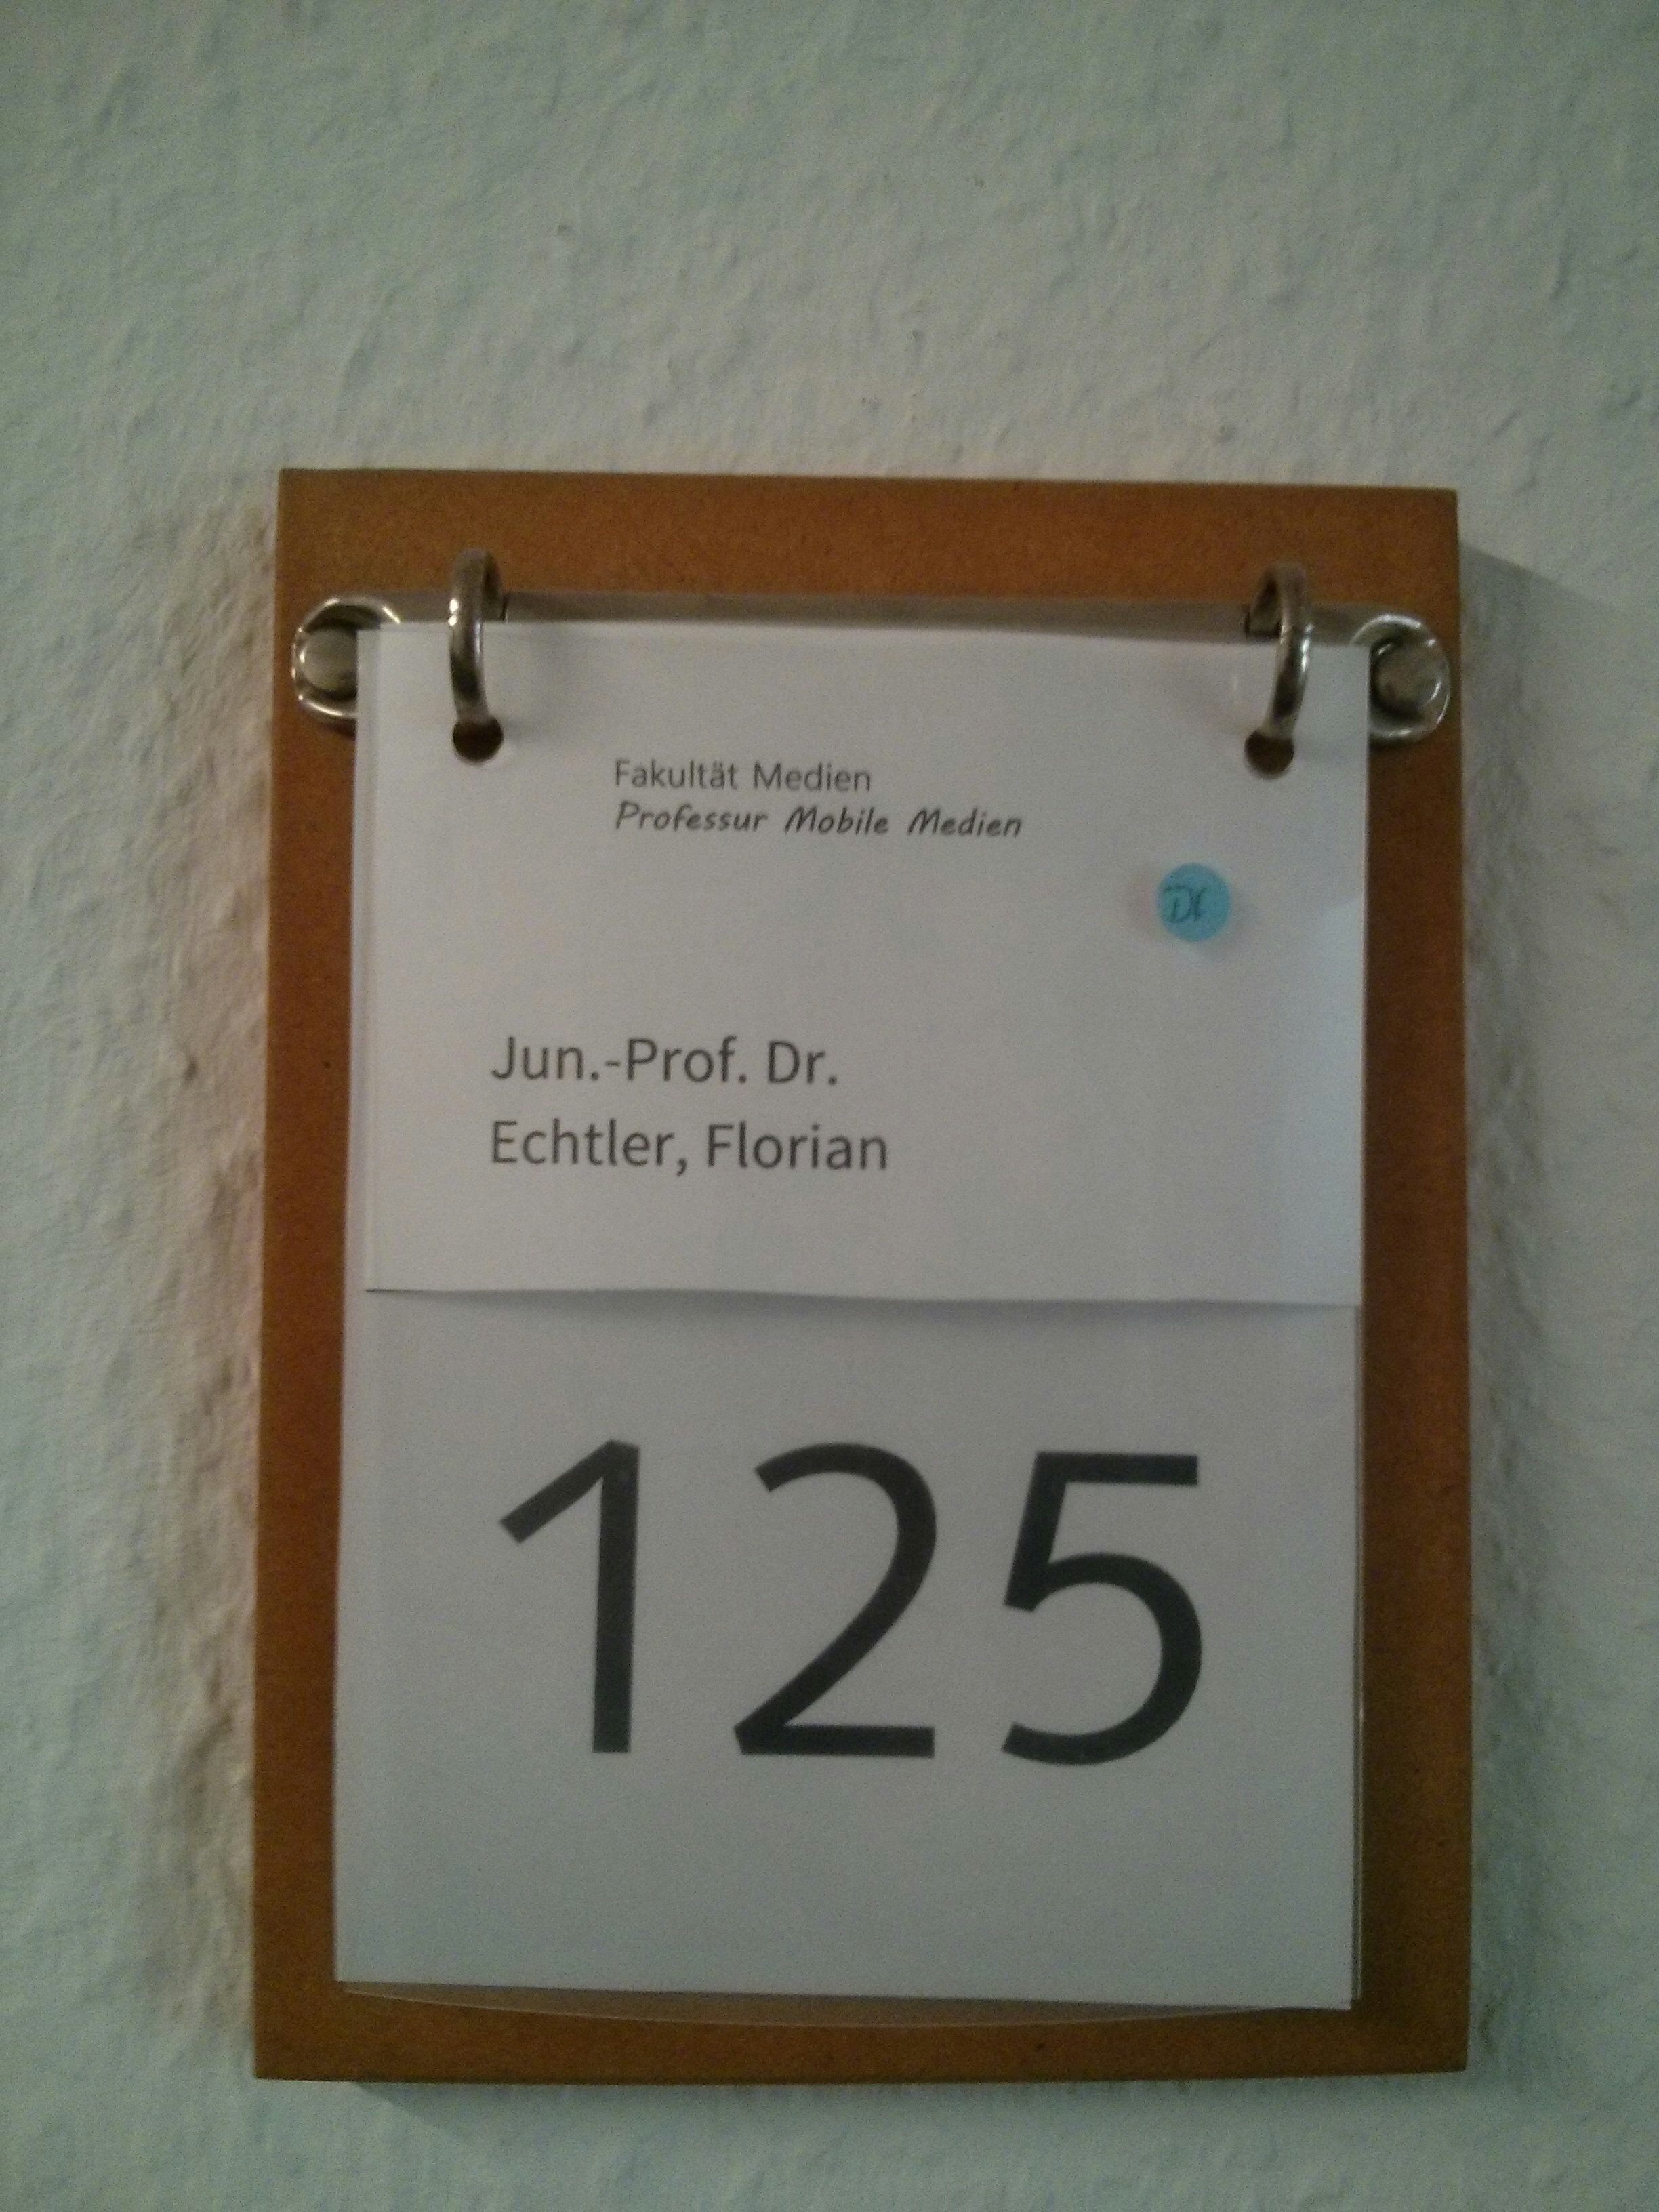
\includegraphics[width=0.34\textwidth]{./img/Tuerschild.jpg}
      \label{img:tuerschild}
    }
    \subfigure[Ein Türschild mit Board]{
      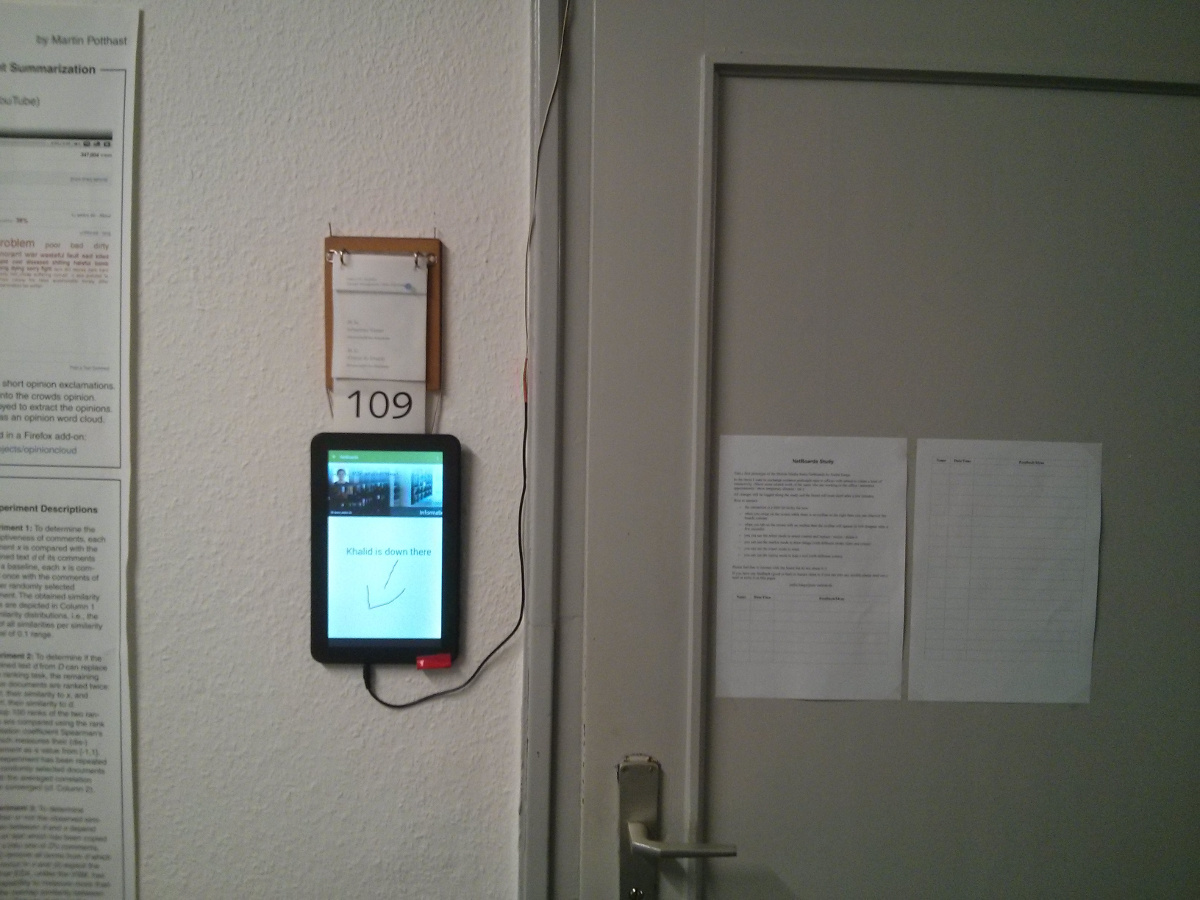
\includegraphics[width=0.605\textwidth]{./img/experiment01.jpg}
      \label{img:experiment01}
    }
  \caption{Versuchsaufbau des Experiments}
  \label{img:Versuchsaufbau}
\end{figure}
\\
Da sich die Rückwand des Tablets abschrauben ließ, konnte ich zwei Löcher hinein bohren. Diese dienten zur Anbringung eines Drahtes, welcher über das Türschild gehängt werden konnte. Für das Experiment war diese Aufhängung vollkommen ausreichend.
\\
Für die Stromversorgung wurde das Ladekabel des Tablets verlängert, damit es an eine Steckdose im Büro angeschlossen werden konnte.
\\
Als Testnutzer für das Experiment konnte ich zwei Mitarbeiter der Professur für Webtechnologien und Informationssysteme gewinnen.
Diese Nutzer teilten sich ein Büro, wodurch nur ein Anzeigegerät benötigt wurde.
Nach einer Einweisung zur Benutzung des Systems stellte sich heraus klar, dass beide Tester nicht mit der Interaktivität der Boards einverstanden waren.
Jeder Gast konnte den dargestellten Inhalt beliebig ändern.
Durch die Anonymität der Gäste hätte es zu missbräuchlicher Nutzung und Vandalismus kommen können.
% Hier Beispiel mit Mensa Kinderhacksteak anstelle Rinderhacksteak
Aus diesem Grund habe ich für die Nutzer zwei verschiedene Ansichten erstellt:
\begin{itemize}
  \item eine Backend-Sicht, auf der sie ihre Änderungen machen konnten
  \item eine Frontend-Sicht, die auf dem Tablet angezeigt wurde, nach 5 Minuten den aktuellen Stand abspeicherte und die Sicht auf den aktuellsten Stand der Backend-Sicht setzte
\end{itemize}
% \begin{figure}[h!]
%   \centering
%     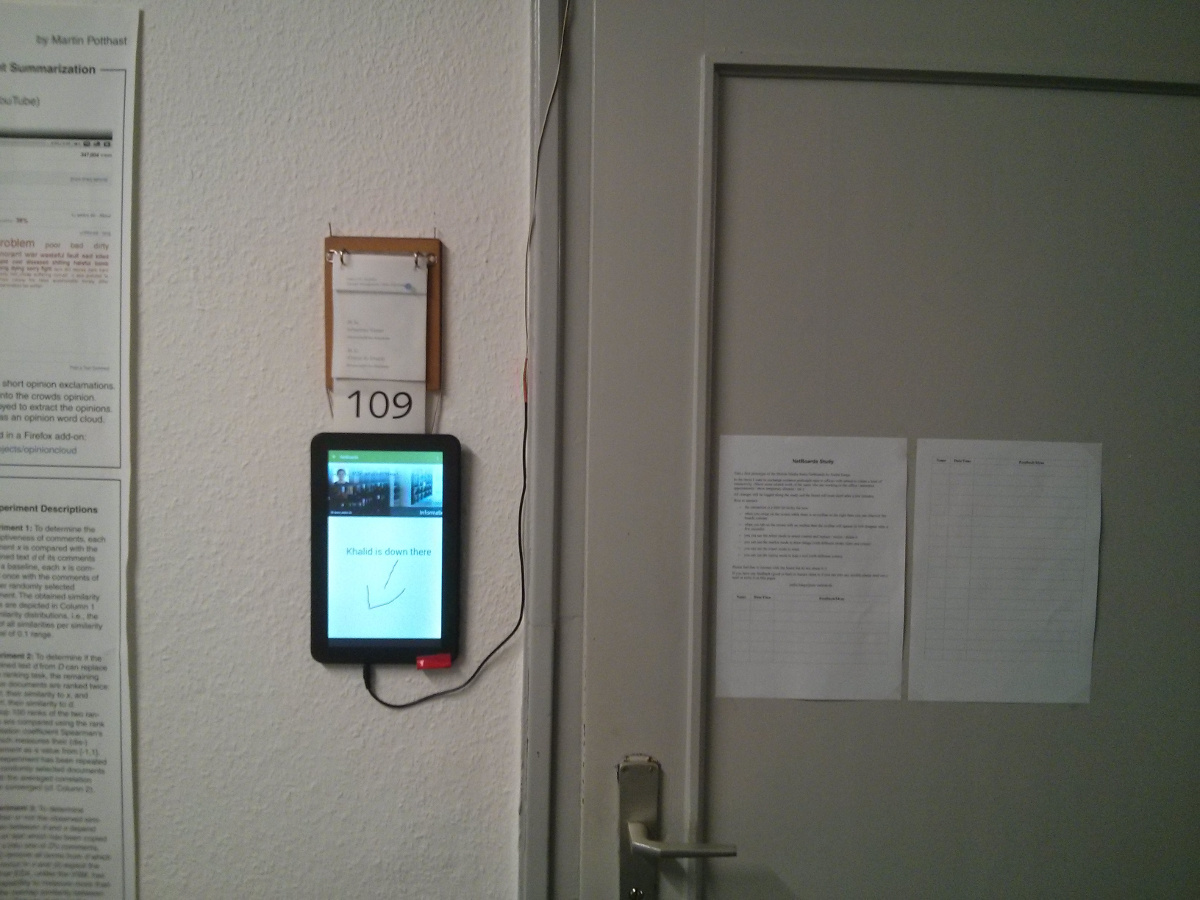
\includegraphics[width=0.7\textwidth]{./img/experiment01.jpg}
%   \caption{Versuchsaufbau des Experiments}
%   \label{img:experiment01}
% \end{figure}



% Experiment Dauer
% 28.05.2015 - 08.06.2015
% 12 Tage
\section{Auswertung}\label{AuswertungVorstudie}
Das Experiment lief 12 Tage. Die Nutzer erstellten sich zu Beginn jeweils einen Nutzeraccount und richteten ihr Board ein. Jeder der beiden lud ein Profilbild hoch und gab seinen Namen sowie seinen akademischen Grad an.
Einer der Tester benutzte das Display um das Banner der Professur zu präsentieren \abb{img:experiment02} und um Gäste \bspw darüber zu informieren, dass er sich zur Zeit im Büro befand \abb{img:experiment03}.
\\
Positiv war, dass das Board viel Aufmerksamkeit zu erzeugen schien. Viele vorbeigehende Nutzer blieben stehen, um sich das Display genauer anzusehen und interagierten sogar damit. Somit entstanden viele Zeichnungen, wovon viele leider keinen tieferen Sinn hatten wie \bspw die Zeichnung in Abb. \ref{img:experiment04}. Jedoch gab es auch ab und an Nachrichten, die direkt an die Besitzer des Boards gerichtet waren, wie das Bild einer Kaffeetasse mit einem Fragezeichen aus Abb. \ref{img:experiment05}, was die Frage nach einer Kaffeepause darstellen sollte.
\begin{figure}[h!]
  \centering
    \subfigure[erste Änderung der Nutzer]{
      \frame{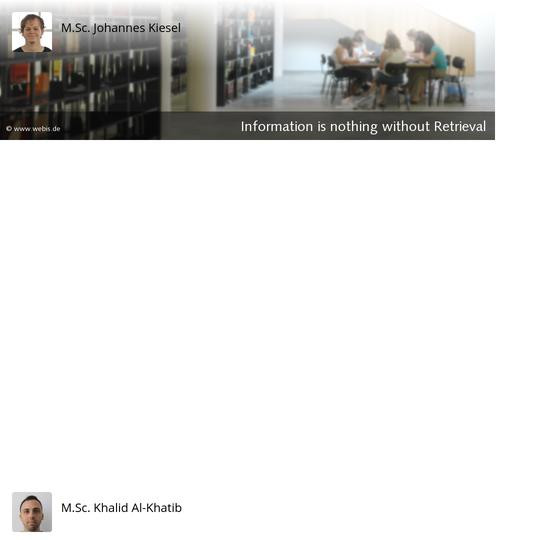
\includegraphics[width=0.4\textwidth]{./img/experiment02_empty.jpg}}
      \label{img:experiment02}
    }
    \subfigure[Statusangabe eines Nutzers]{
      \frame{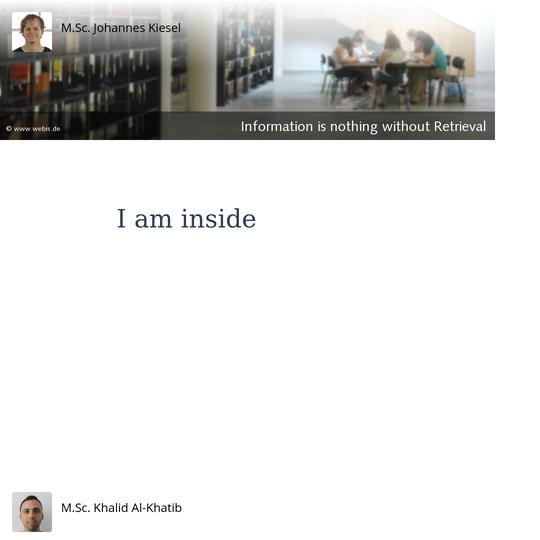
\includegraphics[width=0.4\textwidth]{./img/experiment03_statusContent.jpg}}
      \label{img:experiment03}
    }
    \subfigure[gezeichnetes Bild eines Gastes]{
      \frame{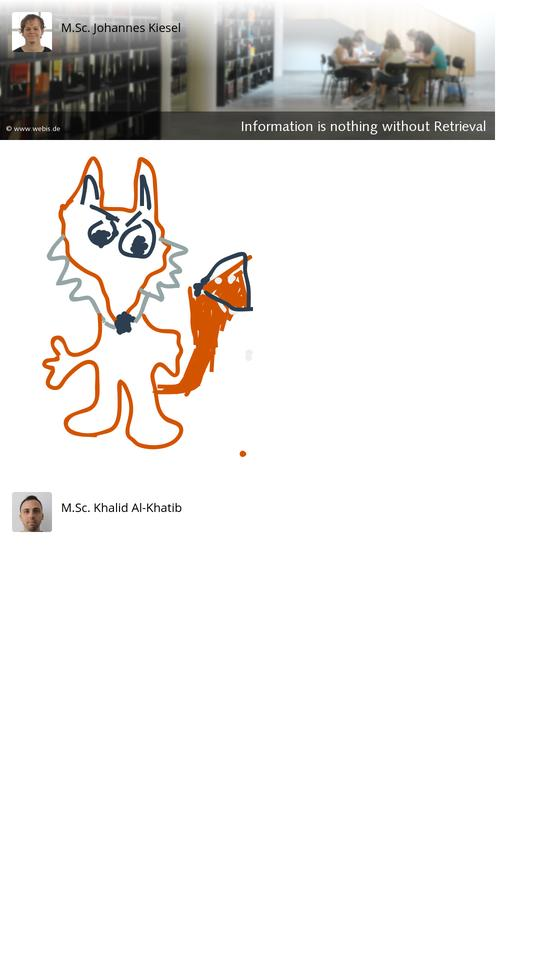
\includegraphics[width=0.4\textwidth]{./img/experiment04_fox.jpg}}
      \label{img:experiment04}
    }
    \subfigure[Frage eines Gastes]{
      \frame{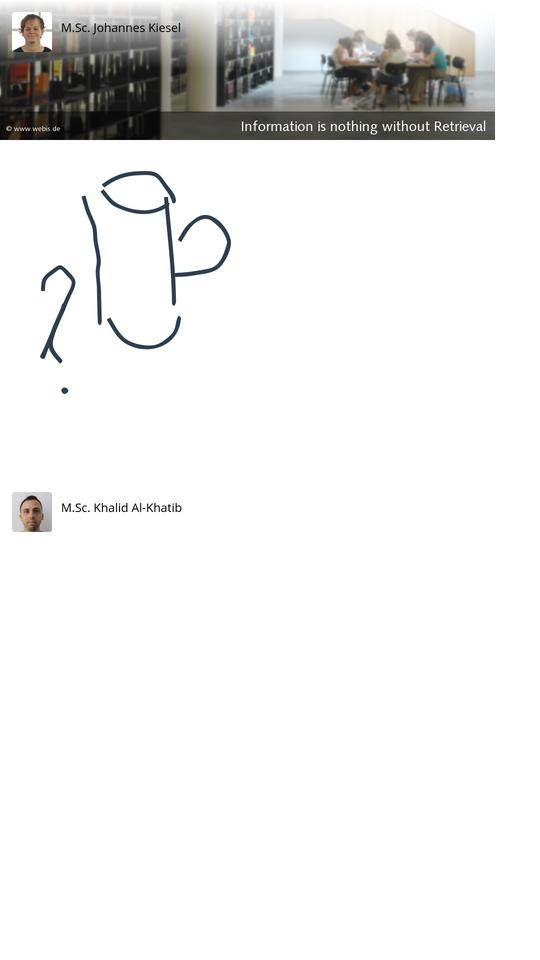
\includegraphics[width=0.4\textwidth]{./img/experiment05_coffee.jpg}}
      \label{img:experiment05}
    }
  \caption{Einige Beispielbilder}
\end{figure}
\\
\\
Nach Beendigung des Experiments führte ich ein Gespräch mit den Testnutzern sowie mit einigen Gästen.
\\
Es stellte sich dabei heraus, dass durch die geringe Auflösung des Tablets den meisten Besuchern gar nicht bewusst wurde, dass zwei Nutzer auf dem Board angemeldet waren. Man musste manuell in der Ansicht scrollen, um den Inhalt des zweiten Nutzers einsehen zu können. Jedoch war auch das ein Problem, da Scrolling nur bei ausgeblendeter Sidebar möglich war. Die meisten Nutzer interagierten demnach nur mit der oberen Hälfte des eigentlichen Inhalts.
\\
Ein weiteres Problem: das Tablet hatte eine sehr geringe Leistung und das Touch-Interface war nicht sehr genau. Deshalb waren Interaktionen mit dem Board sehr langsam und ruckelig.
\\
Positive Äußerungen gab es bezüglich angezeigter Statusmeldungen, wie \bspw ``I am inside''. Die meisten Besucher fanden diese Meldung hilfreich, weil sie deshalb wussten, ob der Mitarbeiter zur Zeit im Raum war.
Weil zum Empfangen einer Benachrichtigung eine Browser-App erforderlich war, hatten sie keine Möglichkeiten darüber benachrichtigt zu werden, wenn jemand etwas auf ihrem Board änderte. Das war den Testern leider nicht bewusst.
Besser wäre es gewesen, wenn die Besitzer eine Email erhalten hätten, sobald ihnen jemand etwas mitteilen wollte.
\\
\\
Als Schlussfolgerung des Experimentes entschied ich mich dazu, ein eigenes System zu entwerfen.
Es war Sinnvoller, dieses System nach den benötigten Anforderungen zu entwickeln, anstatt das NetBoards System so anzupassen, dass es die Anforderungen erfüllte.
\\\todotext{nächster satz mit dieses}
Dieses sollte gut auf Tablets laufen und für eine kleinere Bildschirmgröße angepasst sein. Es erforderte, dass jeder Nutzer eine eigene Sicht bekam, da ansonsten auf dem Tablet zu wenig Platz wäre.
Nur die Besitzer durften die Möglichkeit bekommen, den angezeigten Inhalt zu ändern.
Den Besuchern musste es dennoch möglich sein, mit den Besitzern in Kontakt zu treten, welche darauf eine Benachrichtiguns-Email erhalten sollten.
\\\todotext{abschlusssatz?}